\documentclass[twocolumn]{article}
\usepackage[utf8]{inputenc}

% Macros for citation from ADS
\usepackage{aas_macros}

% Better page spacing
\usepackage{geometry}
\geometry{
    a4paper,
    total={170mm,257mm},
    left=20mm,
    top=20mm
}

% Separation of columns
\setlength{\columnsep}{1cm}

% Automatic spacing of paragraphs, first paragraph indent, and indent size
\usepackage{parskip}
\usepackage{indentfirst}
\setlength\parindent{15pt}

% Include figure files
\usepackage{graphicx}

% Figures and tables using bold fonts
\usepackage[labelfont=bf]{caption}

% Math package
\usepackage{amsmath}

%%%%%%%%%%

% Coding syntax package
\usepackage{listings}
\usepackage{xcolor}

\definecolor{codegreen}{rgb}{0,0.6,0}
\definecolor{codegray}{rgb}{0.5,0.5,0.5}
\definecolor{codepurple}{rgb}{0.58,0,0.82}
\definecolor{backcolour}{rgb}{0.95,0.95,0.92}

\lstdefinestyle{mystyle}{
    backgroundcolor=\color{backcolour},   
    commentstyle=\color{codegreen},
    keywordstyle=\color{magenta},
    numberstyle=\tiny\color{black},
    stringstyle=\color{codepurple},
    basicstyle=\ttfamily\footnotesize,
    breakatwhitespace=false,         
    breaklines=true,                 
    captionpos=b,                    
    keepspaces=true,                 
    numbers=left,                    
    numbersep=5pt,                  
    showspaces=false,                
    showstringspaces=false,
    showtabs=false,                  
    tabsize=2
}

\lstset{style=mystyle}

%%%%%%%%%%

% Hyper links parameters
\usepackage{hyperref}
\hypersetup{
    colorlinks=true,
    citecolor=blue,
    linkcolor=blue,
    filecolor=magenta,      
    urlcolor=blue
}

% Bibliography
\usepackage[round]{natbib}
\bibliographystyle{abbrvnat}

% Author manipulation
\usepackage{authblk}

% Add short title and author
\usepackage{fancyhdr}
\pagestyle{fancy}

% Warning color text
\newcommand{\warning}[1]{\textcolor{red}{\bf #1}}

%%%%%%%%%%%%%%%%%%%%%%%%%%%%%%%%%%%%%%%%%%%%%%%%%%%%%%%%%%%%%%%%%%%%%%%%%%%%%%%%%%%%%%%%%%
%
% PREPARATION
%
%%%%%%%%%%%%%%%%%%%%%%%%%%%%%%%%%%%%%%%%%%%%%%%%%%%%%%%%%%%%%%%%%%%%%%%%%%%%%%%%%%%%%%%%%%

\title{Python introduction}
\author[1]{H.G. Vivien}
\affil[1]{Laboratoire de Physique et Chimie de l'Environnement et de l'Espace (LPC2E), UMR CNRS 7328 - Université d'Orl\'eans, Orl\'eans, France}
\date{\today}
\setcounter{Maxaffil}{0}
\renewcommand\Affilfont{\itshape\small}

\lhead{H.G. Vivien}
\rhead{Python introduction}

%%%%%%%%%%%%%%%%%%%%%%%%%%%%%%%%%%%%%%%%%%%%%%%%%%%%%%%%%%%%%%%%%%%%%%%%%%%%%%%%%%%%%%%%%%
%
% DOCUMENT START
%
%%%%%%%%%%%%%%%%%%%%%%%%%%%%%%%%%%%%%%%%%%%%%%%%%%%%%%%%%%%%%%%%%%%%%%%%%%%%%%%%%%%%%%%%%%

\begin{document}

%%%%%%%%%%%%%%%%%%%%
% Titles, names, abstract, ...
%%%%%%%%%%%%%%%%%%%%

\onecolumn

\maketitle
\hrule

\section*{Introduction}

The following document contains an introduction to the Python programming language, including some lesson about the basics, examples, and exercises. While it can form a useful basis I don't recommend solely relying on it to learn the language; using books and tutorial in parallel is the way to go to learn any language. I recommend particularly the website \href{https://www.learnpython.org/}{https://www.learnpython.org/}, which proposes many interactive tutorials and example.

The following exercises will have a correction uploaded to \href{https://github.com/At0micBee/Exercises}{https://github.com/At0micBee/Exercises}, so that you can check your results and methods to mine. I will try to keep the answer as understandable to beginners as possible, rather than writing to be as efficient as can be.

This document is more centered towards scientific processes and data analysis, and thus might not be suited for other applications. The modules covered will mostly be used for science application, and the exercises require a solid basis in both math and physics. 

\twocolumn

%%%%%%%%%%%%%%%%%%%%
% Rest of the document
%%%%%%%%%%%%%%%%%%%%

\section{Polynomial coefficients}\label{sec:polynomial_coefficients}

The definition of a second order polynomial is:

\begin{equation}\label{eq:poly}
    f(x) = ax^2 + bx + c
\end{equation}

with $a,~b,~c$ real numbers. We're going to look at the impact of changing these coefficients with x in the range $[-10,~10]$. Write a program that will modify each the parameters $a$, $b$ or $c$ independently. Each time we want to produce a figure that shows the resulting polynomial curve for each of the value taken by the variable parameter. Respectively, we want:

\begin{equation}\label{eq:system_polynomial}
    \begin{cases}
        a\in [-1,~1],~b=1,~c=2\\
        a=1,~b\in [-1,~1],~c=2\\
        a=1,~b=2,~c\in [-1,~1]
    \end{cases}\,
\end{equation}

For example, the first case described here would produce Figure.~\ref{fig:polynomial_example}

\begin{figure}
\centering
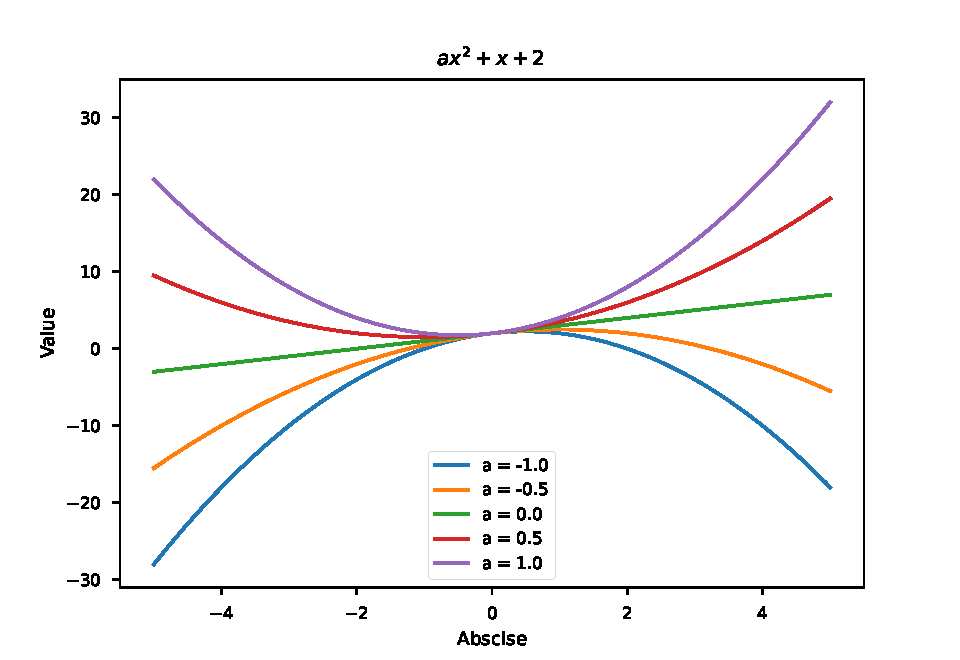
\includegraphics[width=0.5\textwidth]{figures/polynomial_a.pdf}
\caption{Example of solution to Ex.~\ref{sec:polynomial_coefficients}.}
\label{fig:polynomial_example}
\end{figure}

\section{Polynomial roots}\label{sec:polynomial_roots}

Create a program that computes the roots of a polynomial given its parameters $a,~b,~c$, knowing that:

\begin{equation}\label{eq:poly_roots}
    \begin{cases}
        \Delta = b^2 - 4ac\\
        r_\pm = \frac{-b \pm \sqrt{\Delta}}{2a}
    \end{cases}
\end{equation}

\begin{enumerate}
    \item Compute $\Delta$, and figure out if the solution is real or complex
    \item If it is real, solve it, otherwise print a message saying we won't compute it
    \item As a bonus, add another if case to compute when $\Delta=0$, and where $r=\frac{-b}{2a}$
\end{enumerate}

\section{Factorial function}\label{sec:factorial}

Implement a function that takes in an \verb|integer| and returns the result of the factorial of that number, knowing that the factorial function is:

\begin{equation}\label{eq:factorial}
    n! = \prod_{i=1}^n i
\end{equation}

Have it display the result for a few values. Once that is done, we want to look at the trend of this function. To achieve this, we want to compute the factorial of all integer up to $10$, and plot the result.

\section{Computing an average}\label{sec:average}

We are given the following set of values:

\begin{lstlisting}[language=Python]
v = [2.5, 3.2, 4.1, 0.8, 1.2, 2.4]
\end{lstlisting}

Copy this line to a program, and compute both the sum and the average value of this list, with the general form of the sum and average being:

\begin{equation}
    s = \sum_{i=1}^{n} f(i)
\end{equation}

\begin{equation}\label{eq:average}
    a = \frac{1}{n}\sum_{i=1}^{n} f(i)
\end{equation}

Where $n$ is the number of values to take into account, $i$ in the index of the values, and $f(i)$ is the value at index $i$.

\section{Vector manipulation}\label{sec:vector_manip}

Create two vectors of three elements $\Vec{v_1}$ and $\Vec{v_2}$ as follows:

\begin{equation}
    \overrightarrow{v_1}=\begin{pmatrix}
        0.2\\
        1.3\\
        7.4
    \end{pmatrix},~\overrightarrow{v_2}=\begin{pmatrix}
        -7.1\\
        2.4\\
        -0.7
    \end{pmatrix}
\end{equation}

Compute the following:
\begin{enumerate}
    \item The addition $\overrightarrow{v_{\mathrm{add}}} = \overrightarrow{v_1} + \overrightarrow{v_2}$
    \item Multiply them by a scalar: $2\overrightarrow{v_1}$ and $-3\overrightarrow{v_2}$
    \item Combine them: $\overrightarrow{v_{\mathrm{tot}}} = 2\overrightarrow{v_1} - 3\overrightarrow{v_2}$
    \item Compute the scalar product: $S = \overrightarrow{v_1}\cdot\overrightarrow{v_2}$
    \item Compute the rotational: $\overrightarrow{v_{\mathrm{rot}}} = \overrightarrow{v_1}\wedge\overrightarrow{v_2}$
\end{enumerate}

Reminder about the $\overrightarrow{curl}$ product between two vectors:

\begin{equation}
     \overrightarrow{v_1}\wedge\overrightarrow{v_2} = \begin{pmatrix}
        v_{1y}v_{2z} - v_{2y}v_{1z}\\
        v_{1z}v_{2x} - v_{2z}v_{1x}\\
        v_{1x}v_{2y} - v_{2x}v_{1y}
    \end{pmatrix}
\end{equation}

\section{Gravity}\label{sec:gravity}

Consider the force of gravity on a 1 dimensional axis, with $g=9.81\mathrm{m.s^{-1}}$. We want to compute the velocity and position of an object under this gravity field for 10 seconds. Assume the original position is the origin, and that it has no initial velocity.

Once that is done, we want to visualize the movement and speed on a plot to give us an idea of what is happening. Create a plot to represent both the velocity and position in function of time (see Figure.~\ref{fig:gravity_example} for an example).

\begin{figure}
\centering
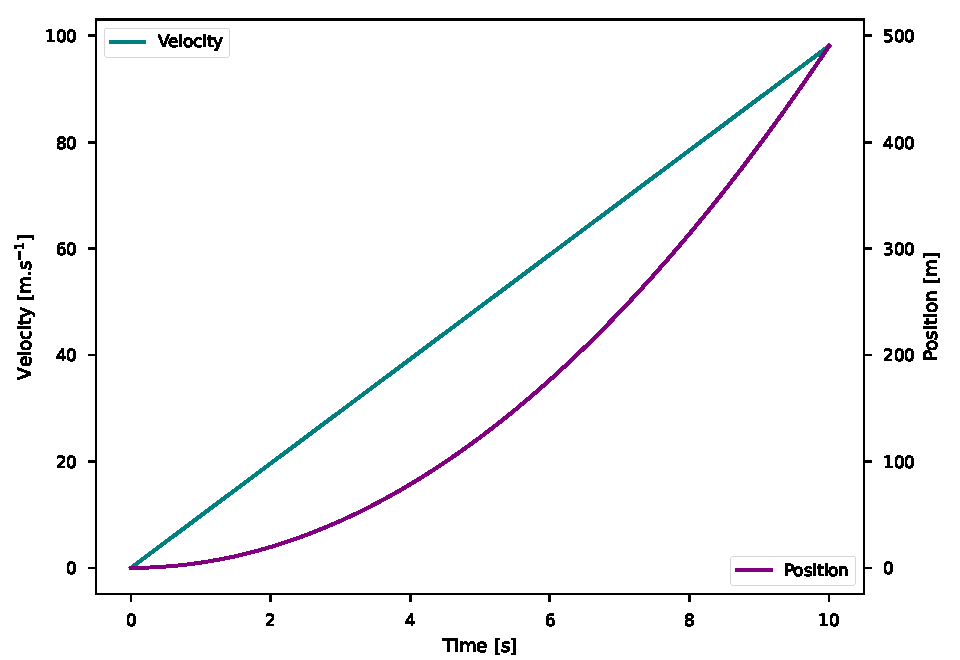
\includegraphics[width=0.5\textwidth]{figures/gravity.pdf}
\caption{Plot showing the solution of Ex.~\ref{sec:gravity}. The velocity is read on the left and position on the right.}
\label{fig:gravity_example}
\end{figure}

\section{Surface areas}\label{sec:surfaces}

Create a function that returns the surface of a circle for a given radius $r$, and one that returns the surface of a square of side $a$. Compute the respective results for $a=r$ for a few values between $0$ and $2$.

Plot the results to visualize the difference of growth between the two.

\section{Gravity, medium difficulty}\label{sec:gravity_medium}

Compute the force between the sun and an Earth mass planet for distances between $0.3$ and $5\mathrm{AU}$. We have $M_\odot = 1.989\cdot10^{30}\mathrm{kg}$, $M_\oplus = 5.972\cdot10^{24}\mathrm{kg}$, $1\mathrm{AU} = 150\cdot10^{9}\mathrm{m}$, and with:

\begin{equation}
    F_{\mathrm{grav}} = G\frac{M_1M_2}{r^2}
\end{equation}

Where $G = 6.674\cdot10^{-11}\mathrm{m^3.kg^{-1}.s^{-2}}$ is the gravitational constant, $M_1$ and $M_2$ are the masses of the objects and $r$ is the distance separating them.

\section{Studying infinite series}\label{sec:infinite}

We are first going to look at a simple series, and then work our way towards something more complicated.

\begin{equation}\label{eq:inf_serie_0}
    s = \sum_{n=1}^{\infty} \frac{1}{n}
\end{equation}

We would like to do two things:

\begin{enumerate}
    \item Estimate if it converges, and if it does to what value
    \item Visualize the impact of each term as $i$ grows
\end{enumerate}

Obviously, we cannot cannot compute an infinity of terms, or it would literally take forever, but we can take advantage of the speed of the machine to compute a lot of them. We can start by only computing the first dozen terms, then we can push it to many more to study the series.

Once that is done, we want to try and apply it to something more useful, and so we are going to try and estimate pi. We use the sum presented in Eq.~\ref{eq:inf_series_pi}, and want to do the same data analysis as we did previously with the other series.

\begin{equation}\label{eq:inf_series_pi}
    \pi = 4\sum_{n=0}^{\infty} \frac{(-1)^n}{2n + 1}
\end{equation}

\section{Chemistry reaction}\label{sec:chemistry}

We consider a chemical system with four solvents A, B, X and Y. A and B remain constant through time, but the concentration of X and Y are dependent on the current concentration of all solvents according to the following system:

\begin{equation}
    \begin{cases}
        dX = A - (B + 1)X + X^2Y\\
        dY = BX - X^2Y
    \end{cases}
\end{equation}

Where A, B, X and Y are the respective concentration of the solvent, and $dX$ and $dY$ the kinetic of the reaction at the given concentrations. We want to see how the concentrations of X and Y evolve through time; given $A = 1$, $X = A + \epsilon$, $Y = B / A$ and $\epsilon$ a small value. We want to be able to input the value of B from the terminal to easily change its value manually.

Compute the state of the system using the Euler scheme; which is defined as follows:

\begin{equation}
    x_{i+1} = x_{i} + \frac{\partial x}{\partial t}\Delta t
\end{equation}

Where $x$ is the quantity we are trying to compute, $i$ are the increment of the disretization, and $\frac{\partial x}{\partial t}\Delta t$ is the compute variation of parameter $x$ during $\Delta t$.

\begin{figure*}
\centering
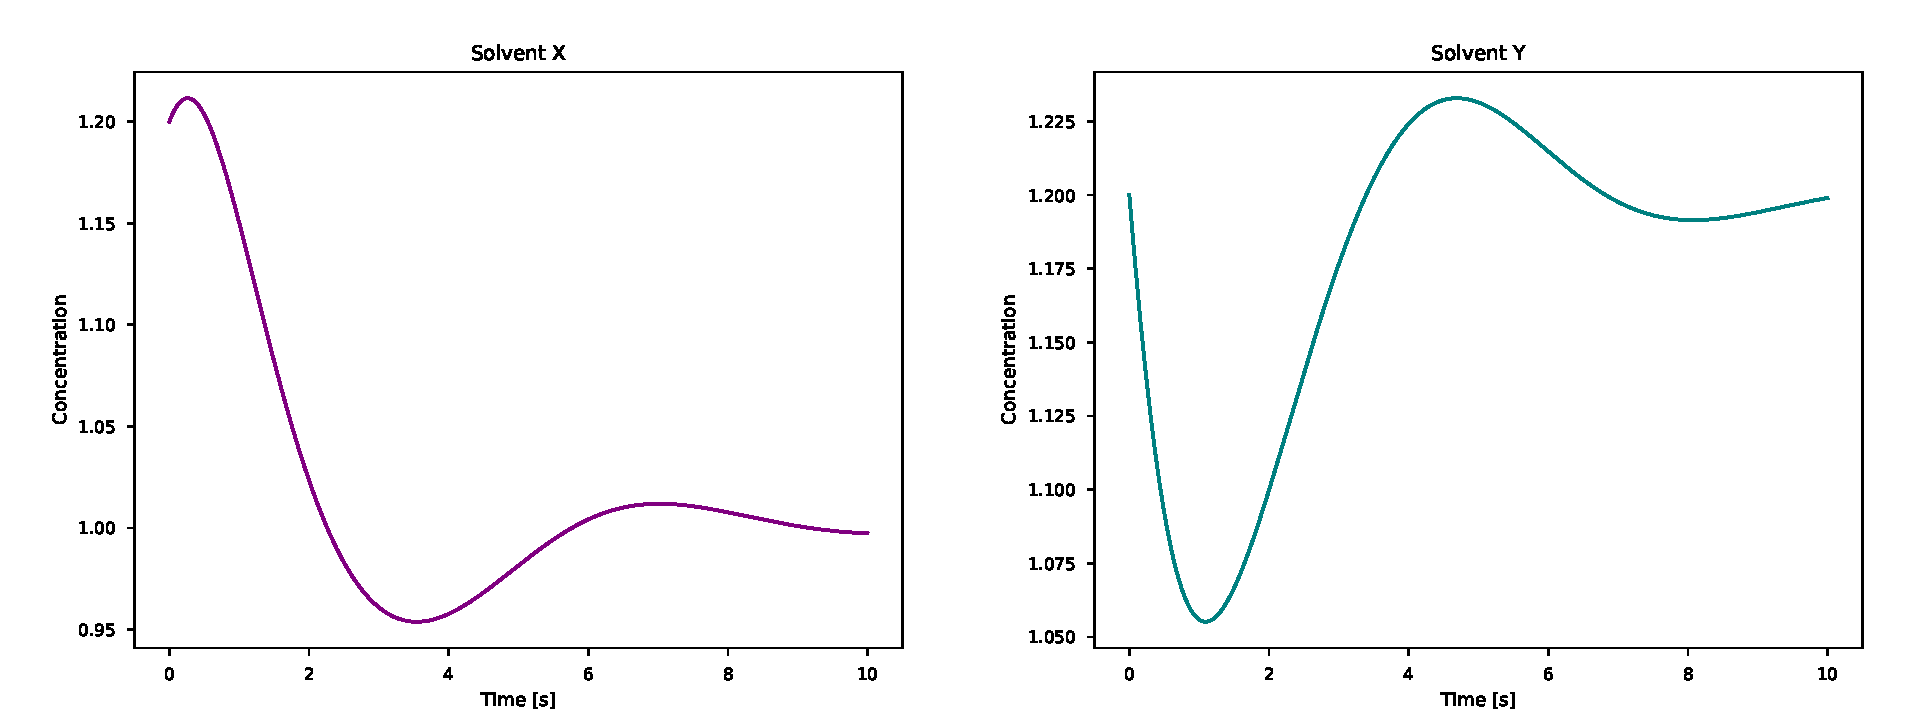
\includegraphics[width=1.0\textwidth]{figures/chemistry.pdf}
\caption{Evolution of the reaction through time using an Euler explicit integration scheme.}
\label{fig:chemical_reaction}
\end{figure*}

\section{Gravity, but complicated this time}\label{sec:gravity_complicated}

We're going to do a similar exercise to the Ex.~\ref{sec:gravity}, but more complicated this time. We're going to compute $g$ at various altitude first, then use that value to compute the motion of a falling object. The general formula to compute gravity is:

\begin{equation}
    g(r) = - \frac{GM(r)}{r^2}
\end{equation}

Where $r$ is the radius at which to estimate the gravity, $G = 6.674\cdot10^{-11}\mathrm{m^3.kg^{-1}.s^{-2}}$ is the gravitational constant and $M$ is the mass under the given radius. Considering that the Earth is a perfect sphere of $6371\mathrm{km}$, that the mass under that radius is of $5.972\cdot10^{24}\mathrm{kg}$ and that the mass of the atmosphere is negligible, compute the gravity for the altitude $z$ between $0$ and $100\mathrm{km}$. \warning{Be careful, the altitude starts at the radius value of $6371\mathrm{km}$!}

We can see that even for a change of only $100\mathrm{km}$, there is a non-negligible change in gravity. Assuming an object starts to fall from an altitude of $100\mathrm{km}$ with no initial velocity, and assuming there is no drag forces in the atmosphere, compute the following:

\begin{enumerate}
    \item The velocity at each point in time during the fall
    \item The position though time
    \item The time it will take to reach the surface
\end{enumerate}

And end the simulation when it hits the ground. To compute each point in time, we're going to use a simple explicit Euler scheme.

\section{Loading data}\label{sec:loading_data}

Download the \verb|N-BK7.dat| file on the Github page, load the data from this file. Plot the variation of the $n,~k$ index in relation to the wavelength.

Once that is done, we are going to see how a change in wavelength influences the medium. We are going to use the Snell-Descartes law (Eq.~\ref{eq:snell_descartes}), and compute the exit angle of a beam of light interacting with the medium.

\begin{equation}\label{eq:snell_descartes}
    n_1\sin(\theta_1) = n_2\sin(\theta_2)
\end{equation}

Where $n_1$ and $n_2$ are the indexes of the incident out outgoing medium, respectively, and $\theta_1$ and $\theta_2$ are the incident and exit angles. We are going to fix $n_1 = n_{\mathrm{air}} \approx 1$ and $\theta_1 = 30^\circ$. We will use the $n$ stored in the file to have a real value for the second medium.

Figure.~\ref{fig:exit_angle} shows what should be obtained, we can see that the exit angle is greatly dependent on the $n$. This is a good illustration of the prism effect.

\begin{figure}
\centering
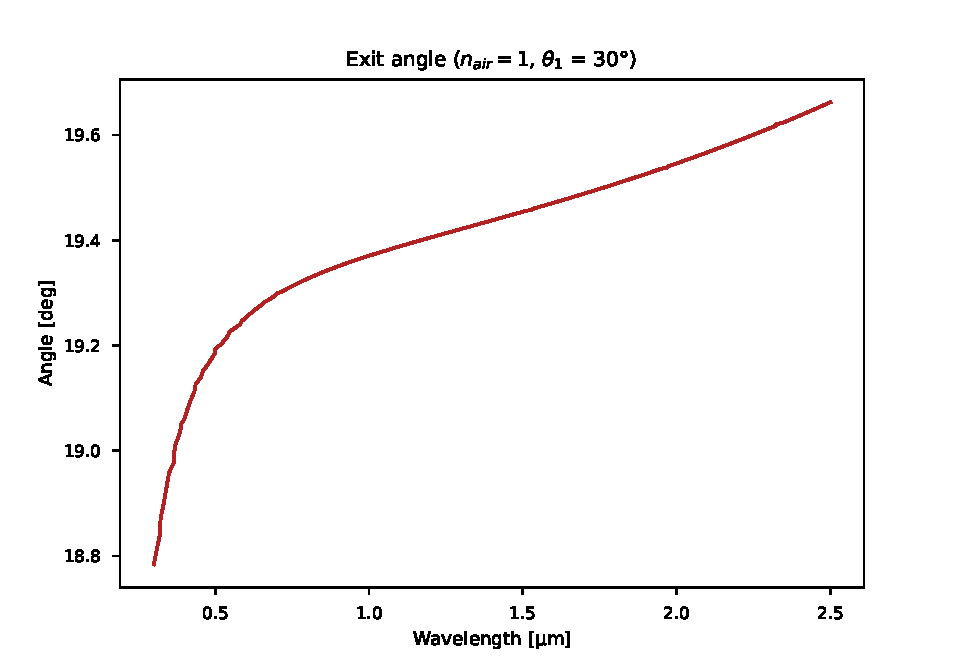
\includegraphics[width=0.5\textwidth]{figures/exit_angle.pdf}
\caption{Illustration of the exit angle depending on the wavelength and $n$ index of the medium.}
\label{fig:exit_angle}
\end{figure}

\section{Planetary properties}\label{sec:planetary_properties}

We have three files from a simulation of planets with a varying amount of water on their surface ($0.01\%$ to $5\%$). We want to first visualize the mass-radius relations of these planets on a plot. Then we want to study the evolution of the parameters in relations to others; namely:

\begin{itemize}
    \item Mass \& gravity
    \item Mass \& pressure
    \item Mass \& radius with atmosphere
    \item $T_{\mathrm{eff}}$ \& $T_{\mathrm{surf}}$
    \item Pressure \& $T_{\mathrm{surf}}$
\end{itemize}

Start by doing it for a single file, then implemented an automated method to do it to all files at the same time.

\section{Spectral analysis}\label{sec:spectral_analysis}

The file \verb|all.tab| contains the emission lines from the spectrum from comet 122P/deVico. The file contains multiple columns, but we are only going to focus on the first two, which are respectively the wavelength of the line and its intensity.

First, we want to plot them together to observe the general trend. Then, we want to create a second plot representing the proper spectrum of the comet. To do that, we are going to model the rays with Gaussian functions. Assuming a width of $1$, compute each emission lines and group them to create the full spectrum.

\section{Working with date and time}\label{sec:datetime}

We are going to go over the basics of the \verb|datetime| module capabilities through the exercise.

First, we want to compute the time elapsed since your birthday. Second, we want to compute the time in six hours from now. Third, we want to compute the sum of two time deltas, to ensure that it is possible.

Finally, we want to load the file named \verb|dates.dat|, and convert its content to proper dates using the \verb|datetime| module. Then, using a delta, we want to check which dates, if any, are within $365$ days from now. (Then test a few other time deltas to make sure it works as desired).

\section{Database with Pandas}\label{sec:database_pandas}

\verb|Numpy| isn't the only module allowing to work with saved data, \verb|Pandas| is another very useful and powerful tool. It is more centered toward very large databases, and has its own format to handle them called \verb|dataframes|.

We are going to look at the Mie scattering from NB-K7 glass for multiple wavelength and particle sizes. We want to plot the results of the scattering on a graph with the wavelength as abscissa and the intensity as ordinate. Each wavelength is in a different file, and can thus be easily plotted one by one.

The \href{https://pandas.pydata.org/}{pandas}\footnote{https://pandas.pydata.org/} documentation is very thorough and will help you understand the parallel between it and the way \verb|numpy| works. The correction example given will also help show how the module works.

\section{Numpy and Pandas}\label{sec:numpy_and_pandas}

This exercise's goal is to compare the two modules by doing the same task with both. We have three files containing data about the shape of laser beams, and want to compare them.

In both approaches; load the data into Python, and plot it to represent against the camera position:

\begin{itemize}
    \item The width
    \item The thickness
    \item The power
\end{itemize}

Try to do so on the same graph later, as a sub-part of the exercise.

\newpage
\appendix

\section{Terminology}\label{app:tarminology}

In this section, we go over some of the terminology and notation related to Python and programming in general.

\begin{itemize}
    \item \emph{Data type}: Also sometimes referred to simply as \emph{type}, it is the nature of some data in the code. For example $6$ would be an \verb|integer|, and \verb|[4.2, 6.5, 2.8]| is a \verb|list| of \verb|float|.
    \item \emph{Keyword}: In a programming language, a \emph{keyword} is a word reserved for a specific use by the language. For example, \verb|while| is a \emph{keyword}.
    \item \emph{Variable}: A \emph{variable} is a container for a value within the program. It can store many different values of a \emph{data type}.
    \item \emph{Function}: As in mathematics, a \emph{function} is a process that does something. Usually it acts on data within the code to either change it, or produce a result based on it.
    \item \emph{Block of code}: Also referred to as \emph{code block} or just \emph{block} sometimes. It is used to described a bit of code that does a specific thing on its own.
    \item \emph{Declaration}: When we create a \emph{function} or \emph{variable}, we call that the \emph{declaration}. It is an easy way to refer to the original instantiation of a bit of code. It is also under certain circumstances called \emph{implementation}.
\end{itemize}

\section{Modules}\label{app:modules}

There are a lot of modules available to do a multitude of things in Python. We are mostly focusing on math, physics and data analysis, and for that there are a few key modules that are likely to be used very often:

\begin{itemize}
    \item \verb|numpy|: Math and array / matrices
    \item \verb|pyplot|: Data visualization
    \item \verb|pandas|: Dataframe, easy data handling
    \item \verb|json|: JSON format reader and writer
\end{itemize}

If a module isn't installed, it can easily be installed using the Python \verb|pip| tool. To install any Python module, open a terminal and use the following command:

\begin{lstlisting}
pip install <module>
\end{lstlisting}

Where \verb|<module>| is the name of the name of the module to be installed. Once a module is installed, it can be used by the python interpreter, but it doesn't mean the interpreter \emph{knows} that is has to use it when running a given program file. To tell it that it is the case, it is necessary to \verb|import| the required module in the file. To do that, we use the \verb|import| command:

\begin{lstlisting}[language=Python]
import numpy as np
\end{lstlisting}

In the previous example, we \verb|import| the \verb|numpy| module to be used in the program. The \verb|as| \emph{keyword} allows us to create an alias name for a module, to simplify the notation later on.

\section{Conditional statements}

Effectively, these are tests that the program looks at, and is able to execute a certain \emph{block of code} in function of the result of the test. They are also called \verb|if|/\verb|else| statements. The semantics of a conditional statement is the call to the right \emph{keyword}, then the Boolean test, then the \emph{block of code} to execute if the result is \verb|True|.

In the following example, we look at an arbitrary variable \verb|a| and check to see what values it possesses.

\begin{lstlisting}[language=Python]
if a < 5:
    print("a is smaller than 5!")
elif a > 15:
    print("a is larger than 15!")
else:
    print("a is between 5 and 15!")
\end{lstlisting}

\section{Loops}\label{app:loops}

Loops allow us to go over the same \emph{block of code} and varying only a parameter at each iteration. The idea behind it is simple, we create some condition that will change iteratively, so that we don't have to write the same thing multiple times.

\begin{lstlisting}[language=Python]
for i in range(0, 50, 1):
    print("The square of", i, "is", i**2)
\end{lstlisting}

In the example above, we compute the square of the first 50 integers. If we didn't use a \verb|for| loop, we would have needed to write manually the operation for each number. A very important thing to understand, is that the \verb|for| loop requires an object that is \emph{iterable}. That means that the object used must offer multiple values, so that each iteration can take place in a meaningful way.

There are other ways to create loops, we can for example use the \verb|while| loop, which uses a condition to establish whether or not the next iteration will happen or not.


\section{Simple examples}

\subsection{Declaring a variable}

A \emph{variable} stores some data for us, so that we don't have to worry about it ourselves. It can hole multiple \emph{types}, and can be \emph{declared} in a number of ways. Usually, we will simply give it a name, and tell it what to store directly.

\begin{lstlisting}[language=Python]
import numpy as np

# Two examples where we give a value manually
some_number = 3.548
some_text = "This is a a text!"

# Giving a value through a function
an_array = np.linspace(0, 10, 2500)
\end{lstlisting}

\subsection{Declaring a function}

To \emph{declare} a \emph{function}, we need to use the \verb|def| \emph{keyword}. We then need to specify a name for our \emph{function}, as well as explicitly tell whether or not it has some input values. The line is terminated with a column, and the lines belonging to the \emph{function} process have to be indented once. At the end of the \emph{function}, we have the option to \verb|return| something out of this process.

For example, we can create a function that returns a polynomial based on input coefficients and point at which to estimate the function.

\begin{lstlisting}[language=Python]
# Defining the polynomial function
def poly(a, b, c, x):
    return a * x**2 + b * x + c

# Storing the return value to a variable
res = poly(2, -3, 7, 2.5)
\end{lstlisting}

In this example, the \emph{function} \verb|poly| computes the value of the polynomial $f(x) = 2x^2 - 3x + 7$ at $x=2.5$. Because the function has a \verb|return| value, we can store it to a \emph{variable} to use it later on (in a \emph{variable} called \verb|res| in the example).

\subsection{Append to list}\label{app:append}

To append a value at the end of a list, there is a \emph{function} called \verb|.append()| that let's us do just that. It can any list \verb|ls| of length $n$, and create the $n+1$ index and assign it a value.

\begin{lstlisting}[language=Python]
ls = [42, 56, 84]   # List of length 3

ls.append(-10)      # Appending -10

print(ls)           # List is now length 4
\end{lstlisting}

In the previous example, we have a list of length 3 (max index = 2), and we wanted to create index 3 with a value of $-10$. Using the \verb|.append()| \emph{function} allows us to do so very easily. Importantly, it also allows us to create a list of identical dimension to a reference when in a \verb|for| loop. By creating an empty list, and appending a given value at each pass, we will obtain a lisst of identical length to our reference one.

\begin{lstlisting}[language=Python]
# Creating a list of length 6, and an empty one
x = [0.0, 0.1, 0.2, 0.3, 0.4, 0.5]
y = []

# Going through the values of the first
# and appending to the second one
for value in x:
    y.append(value**2)

# List y is now length 6
print(y)
\end{lstlisting}

In the previous example, we compute the square of some value in a list that has a fixed length (here 6). Because this list (\verb|x|) could have unknown length, we create and empty list (\verb|y|) to store the result at each point, and need to fill it accordingly. To do so, we go through our reference list \verb|x|, which contains the values we want to use, and append the result to our second list \verb|y|. Because we appended as many times as there are values in the \verb|x| list, the \verb|y| now has the same length as \verb|x|

\subsection{Plotting some data}\label{app:plots}

The following is a simple example showing how to use \verb|pyplot| and \verb|numpy| to visualize some data. We are going to plot the $\sin$ function for $x\in[-\pi,~\pi]$.

\begin{lstlisting}[language=Python]
# Calling the required modules
import numpy as np
import matplotlib.pyplot as pl

# Creating 1000 values for x in the range
# And taking their sinus values
x = np.linspace(-np.pi, np.pi, 1000)
y = np.sin(x)

# Creating a figure
pl.figure()

# Plotting our data
pl.plot(x, y)

# Useful functions for clarity of plot
pl.title("Sinus function")
pl.xlabel("Value of x")
pl.ylabel("Corresponding sinus value")

# Saving the figure
pl.savefig("sinus.pdf")

# Closing the figure
pl.close()
\end{lstlisting}

%\bibliography{bib.bib}

\end{document}
